\documentclass{beamer}

\usepackage{pgfpages}
\usepackage{caption}
\usepackage{listings}
\usepackage{amsmath}
\usepackage{makecell}
\setbeameroption{show notes on second screen}

\setbeamertemplate{caption}[numbered]
\setbeamerfont{note page}{size=\scriptsize}

\usetheme{Bergen}
\usecolortheme{beetle}

\mode<presentation>

\title{Perbandingan Algoritma \textit{Backtracking} dan Algoritma \textit{Hybrid Genetic} untuk Menyelesaikan Permainan Calcudoku}
\author{Michael Adrian \\ 2013730039 \\ \texttt{michaeladrian39@gmail.com}}
\institute{Program Studi Teknik Informatika \\ Fakultas Teknologi Informasi dan Sains \\ Universitas Katolik Parahyangan}
\date{20 Desember 2017}

\begin{document}

\begin{frame}
\titlepage
\end{frame}

\section{Pendahuluan}

\subsection{Calcudoku}

\begin{frame}
\frametitle{Calcudoku}
\begin{itemize}
\item Salah satu jenis permainan teka-teki aritmatika dan logika
\item Dikenal juga sebagai KenKen, KenDoku, atau Mathdoku
\end{itemize}
\end{frame}

\note{
Calcudoku adalah salah satu jenis permainan teka-teki aritmatika dan \textit{grid}. Permainan ini dikenal juga sebagai KenKen, KenDoku, atau Mathdoku.
}

\begin{frame}
\frametitle{Aturan Permainan}
\begin{itemize}
\item Pemain diberikan sebuah \textit{grid} dengan ukuran \begin{math}n \times n\end{math}
\item \begin{math}n\end{math} biasanya antara 3 sampai dengan 9
\item \textit{Grid} ini harus diisi dengan angka 1 sampai dengan \begin{math}n\end{math}
\item Dalam setiap baris setiap angka hanya muncul sekali
\item Dalam setiap kolom setiap angka hanya muncul sekali
\item \textit{Grid} dibagi ke dalam \textit{cage}
\item \textit{Cage} adalah sekelompok sel yang dibatasi oleh garis yang lebih tebal daripada garis pembatas antar sel dengan angka tujuan dan operator yang telah ditentukan
\item Angka-angka dalam setiap \textit{cage} harus mencapai angka tujuan jika dihitung menggunakan operator yang telah ditentukan
\item Angka tujuan dan operasi yang telah ditentukan ditulis di sudut kiri atas \textit{cage}
\end{itemize}
\end{frame}

\note{
Seperti dalam Sudoku, dalam teka-teki ini, pemain diberikan sebuah \textit{grid} dengan ukuran \begin{math}n \times n\end{math}, dengan \begin{math}n\end{math} biasanya antara 3 sampai dengan 9. \textit{Grid} ini harus diisi dengan angka 1 sampai dengan \begin{math}n\end{math} sehingga dalam setiap baris setiap angka hanya muncul sekali, dalam setiap kolom setiap angka hanya muncul sekali. Perbedaannya dengan Sudoku adalah, Calcudoku dibagi ke dalam \textit{cage} (sekelompok sel yang dibatasi oleh garis yang lebih tebal daripada garis pembatas antar sel dengan angka tujuan dan operator yang telah ditentukan), dan angka-angka dalam setiap \textit{cage} harus mencapai angka tujuan jika dihitung menggunakan operator yang telah ditentukan. Angka tujuan dan operasi yang telah ditentukan ditulis di sudut kiri atas \textit{cage}.
}

\begin{frame}
\frametitle{Operator-Operator Matematika}
\begin{itemize}
\item Ada 5 kemungkinan operator:
	\begin{itemize}
	\item + (penjumlahan)
	\item - (pengurangan)
	\item \begin{math}\times\end{math} (perkalian)
	\item \begin{math}\div\end{math} (pembagian)
	\item = (sama dengan)
	\end{itemize}
\item Jika operasi matematika yang ditentukan adalah pengurangan atau pembagian, maka ukuran \textit{cage} harus berukuran dua sel
\end{itemize}
\end{frame}

\note{
Ada lima kemungkinan operator:
\begin{enumerate}
\item +, sebuah operator \begin{math}n\end{math}-ary yang menandakan penjumlahan.
\item -, sebuah operator biner yang menandakan pengurangan.
\item \begin{math}\times\end{math}, sebuah operator  \begin{math}n\end{math}-ary yang menandakan perkalian.
\item \begin{math}\div\end{math} sebuah operator biner yang menandakan pembagian.
\item =, (simbol ini biasanya dihilangkan), sebuah operator uner yang menandakan persamaan.
\end{enumerate}
Jika operasi matematika yang ditentukan adalah pengurangan atau pembagian, maka ukuran \textit{cage} harus berukuran dua sel. Pada beberapa versi dari teka-teki ini, hanya angka tujuan yang diberikan, dan pemain harus menebak operator dari setiap \textit{cage} untuk menyelesaikan teka-tekinya.
}

\begin{frame}
\frametitle{Contoh Permainan}
\begin{figure}
\centering
\captionsetup{justification=centering}
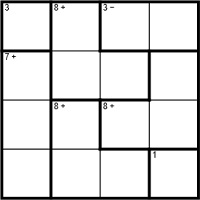
\includegraphics[scale=1]{Gambar/Backtracking1}
\caption[Contoh permainan teka-teki Calcudoku dengan ukuran \textit{grid} 4 x 4 yang belum diselesaikan. ]{Contoh permainan teka-teki dengan ukuran \textit{grid} 4 x 4 yang belum diselesaikan. }
\label{fig:backtracking1}
\end{figure}
\end{frame}

\begin{frame}
\frametitle{Contoh Solusi}
\begin{figure}
\centering
\captionsetup{justification=centering}
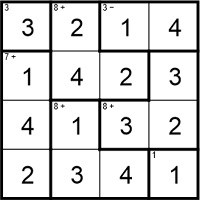
\includegraphics[scale=1]{Gambar/Backtracking2}
\caption[Solusi untuk permainan teka-teki Calcudoku yang diberikan pada Gambar~\ref{fig:backtracking1} ]{Solusi untuk permainan teka-teki Calcudoku yang diberikan pada Gambar~\ref{fig:backtracking1}. }
\label{fig:backtracking2}
\end{figure}
\end{frame}

\subsection{Algoritma \protect\textit{Backtracking}}

\begin{frame}
\frametitle{Algoritma \protect\textit{Backtracking}}
\begin{itemize}
\item Sebuah algoritma umum yang mencari solusi dengan mencoba salah satu dari beberapa pilihan, jika pilihan yang dipilih ternyata salah, komputasi dimulai lagi pada titik pilihan dan mencoba pilihan lainnya
\item Untuk bisa melacak kembali langkah-langkah yang telah dipilih, maka algoritma harus secara eksplisit menyimpan jejak dari setiap langkah yang sudah pernah dipilih, atau menggunakan rekursi (\textit{recursion})
\item Rekursi dipilih karena jauh lebih mudah daripada harus menyimpan jejak setiap langkah yang pernah dipilih
\item Hal ini menyebabkan algoritma ini biasanya berbasis DFS (\textit{Depth First Search})
\end{itemize}
\end{frame}

\note{
Algoritma \textit{backtracking} adalah sebuah algoritma umum yang mencari solusi dengan mencoba salah satu dari beberapa pilihan, jika pilihan yang dipilih ternyata salah, komputasi dimulai lagi pada titik pilihan dan mencoba pilihan lainnya. Untuk bisa melacak kembali langkah-langkah yang telah dipilih, maka algoritma harus secara eksplisit menyimpan jejak dari setiap langkah yang sudah pernah dipilih, atau menggunakan rekursi (\textit{recursion}). Rekursi dipilih karena jauh lebih mudah daripada harus menyimpan jejak setiap langkah yang pernah dipilih. Hal ini menyebabkan algoritma ini biasanya berbasis DFS (\textit{Depth First Search}).
}

\subsection{Algoritma \protect\textit{Hybrid Genetic}}

\begin{frame}
\frametitle{Algoritma \textit{Hybrid Genetic}}
\begin{itemize}
\item Dalam kasus ini, algoritma \textit{hybrid genetic} adalah gabungan dari algoritma \textit{rule based} dan algoritma genetik
\item Algoritma \textit{rule based} akan dijalankan sampai pada titik dimana algoritma tidak bisa menyelesaikan permainan teka-teki Calcudoku
\item Jika algoritma sudah tidak bisa menyelesaikan permainan, maka algoritma genetik akan mulai dijalankan
\end{itemize}
\end{frame}

\note{
Dalam kasus ini, algoritma ini gabungan dari algoritma \textit{rule based} dan algoritma genetik. Algoritma \textit{rule based} akan dijalankan sampai pada titik dimana algoritma tidak bisa menyelesaikan permainan teka-teki Calcudoku. Jika algoritma sudah tidak bisa menyelesaikan permainan, maka algoritma genetik akan mulai dijalankan.
}

\begin{frame}
\frametitle{Algoritma \textit{Rule Based}}
\begin{itemize}
\item Sebuah algoritma berbasis aturan logika untuk menyelesaikan teka-teki Sudoku dan variasinya, termasuk Calcudoku
\item Beberapa aturan logika yang digunakan dalam algoritma ini adalah:
	\begin{itemize}
 	\item \textit{Single square rule}
	\item \textit{Naked subset rule}
	\item \textit{Hidden single rule}
	\item \textit{Killer combination}
	\end{itemize}
\end{itemize}
\end{frame}

\note{
Algoritma \textit{rule based} adalah sebuah algoritma berbasis aturan logika untuk menyelesaikan teka-teki Sudoku dan variasinya, termasuk Calcudoku. Menurut Johanna, Lukas, dan Saputra, beberapa aturan logika yang digunakan dalam algoritma ini adalah \textit{single square rule}, \textit{naked subset rule}, \textit{hidden single rule}, \textit{evil twin rule}, \textit{killer combination}, dan \textit{X-wing} ~\cite{johanna:12:hybrid}.
}

\begin{frame}
\frametitle{Algoritma Genetik}
\begin{itemize}
\item Salah satu teknik heuristik \textit{Generate and Test} yang terinspirasi oleh sistem seleksi alam
\item Perpaduan dari bidang biologi dan ilmu komputer.
\item Algoritma ini memanipulasi informasi, biasanya disebut sebagai kromosom.
\item Kromosom ini meng-\textit{encode} kemungkinan jawaban untuk sebuah masalah yang diberikan.
\item Kromosom dievaluasi dan diberi \textit{fitness value}.
\item \textit{Child chromosome}) diproduksi dengan menggabungkan dua (atau lebih) \textit{parent chromosome}.
\end{itemize}
\end{frame}

\note{
Algoritma genetik adalah salah satu teknik heuristik \textit{Generate and Test} yang terinspirasi oleh sistem seleksi alam. Algoritma ini adalah perpaduan dari bidang biologi dan ilmu komputer. Algoritma ini memanipulasi informasi, biasanya disebut sebagai kromosom. Kromosom ini meng-\textit{encode} kemungkinan jawaban untuk sebuah masalah yang diberikan. Kromosom dievaluasi dan diberi \textit{fitness value} berdasarkan seberapa baik kromosom dalam menyelesaikan masalah yang diberikan berdasarkan kriteria yang ditentukan oleh pembuat program. Nilai kelayakan ini digunakan sebagai probabilitas kebertahanan hidup kromosom dalam satu siklus reproduksi. Kromosom baru (kromosom anak, \textit{child chromosome}) diproduksi dengan menggabungkan dua (atau lebih) kromosom orang tua (\textit{parent chromosome}). Proses ini dirancang untuk menghasilkan kromosom-kromosom keturunan yang lebih layak, kromosom-kromosom ini meng-\textit{encode} jawaban yang lebih baik, sampai solusi yang baik dan yang bisa diterima ditemukan.

}

\begin{frame}
\frametitle{Tujuan}
\begin{itemize}
\item Tujuan dari penelitian ini adalah:
\begin{enumerate}
\item Membuat perangkat lunak permainan teka-teki Calcudoku.
\item Membandingkan performansi algoritma \textit{backtracking} dengan algoritma \textit{hybrid genetic}.
\end{enumerate}
\item Ruang lingkup dari penelitian ini dibatasi oleh batasan-batasan masalah sebagai berikut:
\begin{enumerate}
\item Ukuran \textit{grid} untuk permainan teka-teki Calcudoku adalah antara \begin{math}4 \times 4\end{math} sampai dengan \begin{math}8 \times 8\end{math}.
\item Pada algoritma \textit{rule based}, aturan-aturan logika yang digunakan dibatasi hanya pada aturan \textit{single square}, \textit{naked single}, \textit{naked double}, \textit{hidden single}, dan \textit{killer combination}.
\end{enumerate}
\end{itemize}
\end{frame}

\note{
Tujuan dari penelitian ini adalah:
\begin{enumerate}
\item Membuat perangkat lunak permainan teka-teki Calcudoku yang menerima input berupa soal teka-teki dan mampu menyelesaikan soal teka-teki tersebut menggunakan algoritma \textit{backtracking} dan \textit{hybrid genetic}.
\item Membandingkan performansi algoritma \textit{backtracking} dengan algoritma \textit{hybrid genetic} dalam hal kecepatan dan kesuksesan dalam menyelesaikan Calcudoku.
\end{enumerate}

Ruang lingkup dari penelitian ini dibatasi oleh batasan-batasan masalah sebagai berikut:
\begin{enumerate}
\item Ukuran \textit{grid} untuk permainan teka-teki Calcudoku adalah antara \begin{math}4 \times 4\end{math} sampai dengan \begin{math}8 \times 8\end{math}. 
\item Pada algoritma \textit{rule based}, yang merupakan bagian dari algoritma \textit{hybrid genetic}, aturan-aturan logika yang digunakan dibatasi hanya pada aturan \textit{single square}, \textit{naked single}, \textit{naked double}, \textit{hidden single}, dan \textit{killer combination}.
\end{enumerate}
}

\section{Analisis}

\begin{frame}
\frametitle{Analisis Perangkat Lunak}
\begin{itemize}
\item Perangkat lunak ini akan menerima masukan dalam bentuk \textit{file} yang berisi:
	\begin{enumerate}
	\item Ukuran \textit{grid}
	\item Jumlah \textit{cage}
	\item Matriks \textit{cage assignment}
	\item Matriks \textit{cage objectives}
\end{enumerate}
\item Perangkat lunak ini akan menghasilkan keluaran berupa GUI permainan teka-teki Calcudoku berdasarkan isi \textit{file} yang di-\textit{load} oleh pengguna.
\item Permainan ini dapat diselesaikan oleh pengguna, atau menggunakan salah satu dari dua \textit{solver} yang disediakan. Kedua \textit{solver} tersebut yaitu:
	\begin{enumerate}
	\item Algoritma \textit{backtracking}, dan
	\item Algoritma \textit{hybrid genetic}.
	\end{enumerate}
\end{itemize}
\end{frame}

\note{
Perangkat lunak ini akan menerima masukan dalam bentuk \textit{file} yang berisi:

\begin{enumerate}
\item Ukuran \textit{grid}.
\item Jumlah \textit{cage}.
\item Matriks \textit{cage assignment}, yang merepresentasikan posisi dari setiap \textit{cage} dalam \textit{grid}.
\item Matriks \textit{cage objectives}, yang berisikan angka tujuan dan operasi matematika yang telah ditentukan untuk setiap \textit{cage}.
\end{enumerate}

Perangkat lunak ini akan menghasilkan keluaran berupa antarmuka grafis permainan teka-teki Calcudoku berdasarkan isi \textit{file} yang di-\textit{load} oleh pengguna.

Permainan ini dapat diselesaikan oleh pengguna dengan usahanya sendiri, atau menggunakan salah satu dari dua \textit{solver} yang disediakan. Kedua \textit{solver} tersebut yaitu:

\begin{enumerate}
\item Algoritma \textit{backtracking}, dan
\item Algoritma \textit{hybrid genetic}.
\end{enumerate}
}

\begin{frame}
\frametitle{Diagram \textit{Use Case}}
\begin{itemize}
\item Diagram \textit{use case} berdasarkan skenario-skenario tersebut dapat dilihat pada Gambar~\ref{fig:analisisusecase}.
\end{itemize}
\begin{figure}
\centering
\captionsetup{justification=centering}
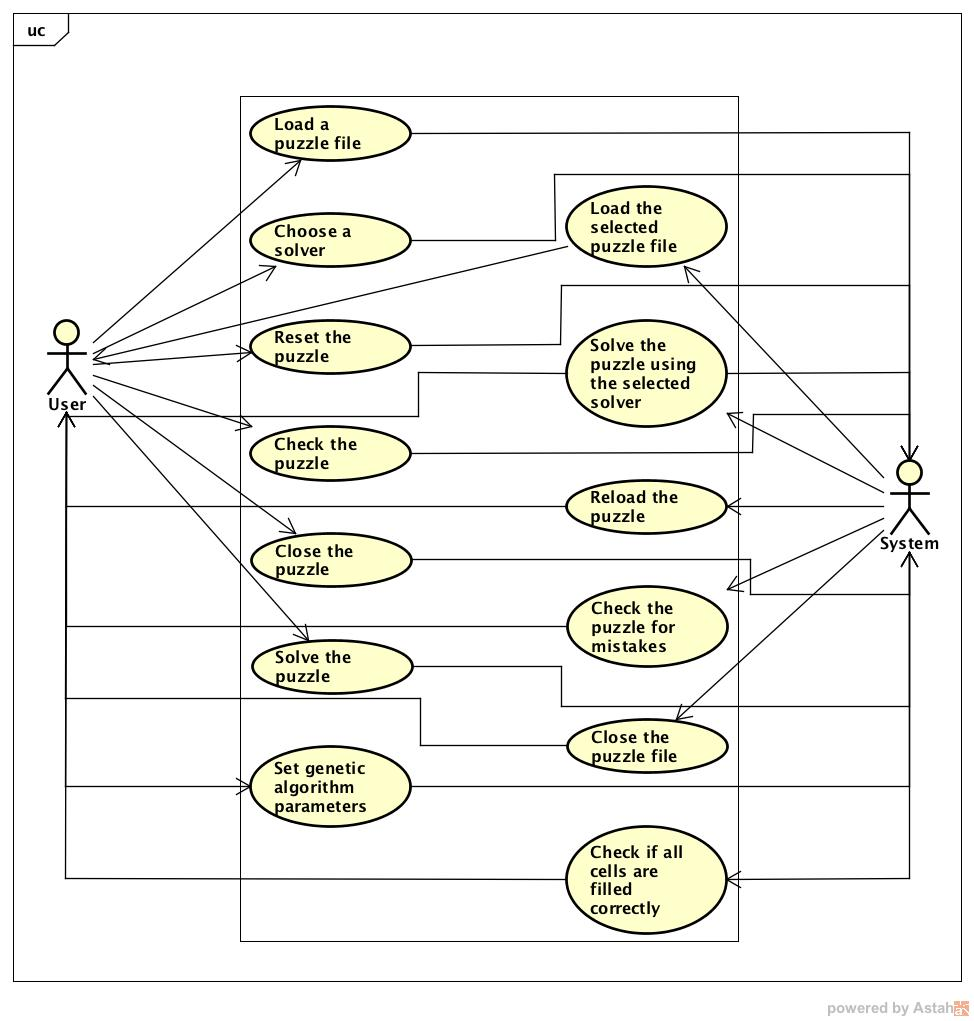
\includegraphics[scale=0.2]{Gambar/Analisis/DiagramUseCase}
\caption[Diagram \textit{use case} untuk perangkat lunak permainan teka-teki Calcudoku]{Diagram \textit{use case} untuk perangkat lunak permainan teka-teki Calcudoku}
\label{fig:analisisusecase}
\end{figure}
\end{frame}

\note{
Diagram \textit{use case} adalah diagram yang menggambarkan interaksi antara sistem (perangkat lunak) dengan pengguna.

Skenario-skenario yang dapat dilakukan oleh pengguna adalah:

\begin{enumerate}
\item Membuka file masukan untuk memulai permainan.
\item Memilih salah satu dari dua \textit{solver} yang disediakan untuk menyelesaikan permainan berdasarkan \textit{file} yang sudah di-\textit{load}.
\item Me-\textit{reset} permainan untuk mengulang permainan berdasarkan \textit{file} masukan yang sudah di-\textit{load} dari awal.
\item Meminta perangkat lunak untuk memeriksa permainan jika ada masukan yang salah di dalam \textit{grid}.
\item Menutup \textit{file} masukan untuk mengakhiri permainan.
\item Menyelesaikan permainan dengan usahanya sendiri.
\item Mengatur nilai dari parameter-parameter untuk algoritma genetik.
\end{enumerate}

Diagram \textit{use case} berdasarkan skenario-skenario tersebut dapat dilihat pada Gambar~\ref{fig:analisisusecase}.
}

\section{Perancangan}

\begin{frame}
\frametitle{Perancangan Masukan}
\begin{itemize}
\item Masukan untuk perangkat lunak Calcudoku ini berupa sebuah \textit{file} teks, seperti yang ditunjukkan pada Gambar~\ref{fig:perancanganmasukan}.
\end{itemize}
\begin{figure}
\centering
\captionsetup{justification=centering}
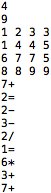
\includegraphics[scale=0.75]{Gambar/Perancangan/PerancanganInput.png}
\caption[Contoh \textit{file} masukan.]{Contoh \textit{file} masukan.}
\label{fig:perancanganmasukan}
\end{figure}
\end{frame}

\note{
Masukan untuk perangkat lunak permainan teka-teki Calcudoku ini berupa sebuah \textit{file} teks, seperti yang ditunjukkan pada Gambar~\ref{fig:perancanganmasukan}.

Adapun rincian dari \textit{file} teks masukan tersebut adalah sebagai berikut:
\begin{enumerate}
\item Baris pertama berisi ukuran \textit{grid} dan banyaknya \textit{cage} dari teka-teki Calcudoku tersebut. Angka pertama adalah ukuran \textit{grid}, dan angka kedua adalah banyaknya \textit{cage}.
\item Baris kedua sampai ke baris ke-\begin{math}2 + (n - 1)\end{math}, dengan \begin{math}n\end{math} adalah ukuran \textit{grid}, berisi matriks \textit{cage assignment}. Matriks ini merepresentasikan posisi dari setiap \textit{cage} dalam \textit{grid}. Setiap \textit{cage} direpresentasikan dengan angka yang berbeda. Setiap \textit{cage} dapat mempunyai ukuran (jumlah sel yang terdapat dalam \textit{cage}) yang bervariasi. Setiap sel dalam sebuah \textit{cage} harus berhubungan secara horizontal atau vertikal dengan sel lain dalam \textit{cage} yang sama.
\item Baris ke-\begin{math}2 + n\end{math} dan seterusnya berisi \textit{cage objectives} untuk setiap \textit{cage}. \textit{Cage objectives} berisikan angka tujuan dan operasi matematika yang telah ditentukan. Angka-angka dalam sebuah \textit{cage} harus mencapai angka tujuan jika dihitung menggunakan operasi matematika yang telah ditentukan.
\end{enumerate}
}

\begin{frame}
\frametitle{Perancangan Keluaran}
\begin{itemize}
\item Keluaran untuk perangkat lunak Calcudoku ini berupa sebuah matriks yang berisi solusi dari teka-teki Calcudoku yang sudah diselesaikan oleh program, seperti dapat dilihat pada Gambar~\ref{fig:perancangankeluaran}.
\end{itemize}
\begin{figure}
\centering
\captionsetup{justification=centering}
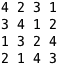
\includegraphics[scale=1]{Gambar/Perancangan/PerancanganOutput.png}
\caption[Contoh keluaran.]{Contoh keluaran.}
\label{fig:perancangankeluaran}
\end{figure}
\end{frame}

\note{
Keluaran untuk perangkat lunak permainan teka-teki Calcudoku ini berupa sebuah matriks yang berisi solusi dari teka-teki Calcudoku yang sudah diselesaikan oleh program, seperti dapat dilihat pada Gambar~\ref{fig:perancangankeluaran}.
}

\begin{frame}
\frametitle{Diagram Kelas}
\begin{itemize}
\item Diagram kelas untuk perangkat lunak ini dapat dilihat pada Gambar~\ref{fig:diagramkelas}.
\end{itemize}
\begin{figure}
\centering
\captionsetup{justification=centering}
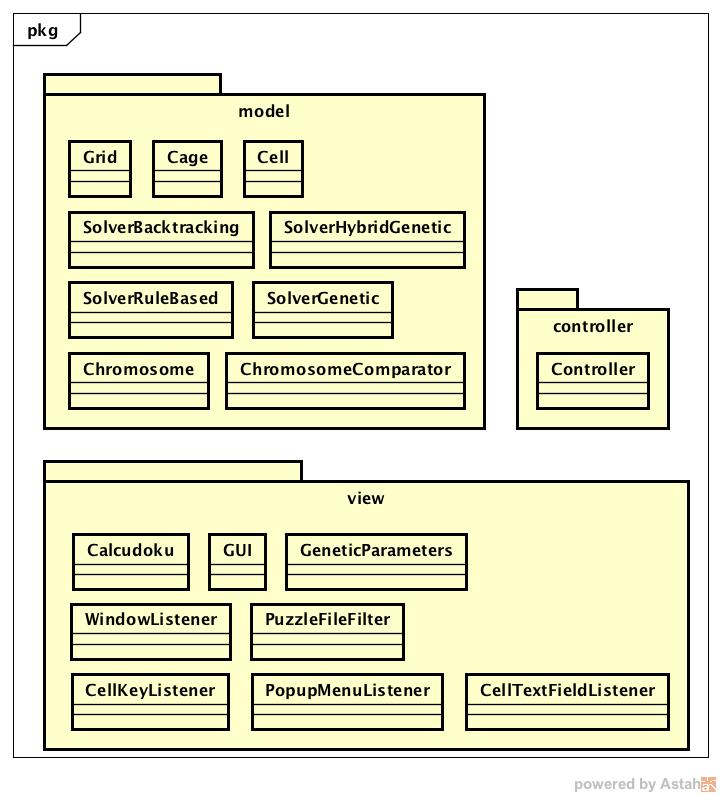
\includegraphics[scale=0.20]{Gambar/Perancangan/DiagramKelas.jpg}
\caption[Diagram kelas untuk perangkat lunak Calcudoku.]{Diagram kelas untuk perangkat lunak Calcudoku.}
\label{fig:diagramkelas}
\end{figure}
\end{frame}

\note{
Diagram kelas untuk perangkat lunak ini dapat dilihat pada Gambar~\ref{fig:diagramkelas}.
}

\section{Kode Program}

\begin{frame}
\frametitle{Kode Program}
\end{frame}

\note{

}

\section{Implementasi dan Pengujian}

\begin{frame}
\frametitle{Hasil Pengujian - Algoritma \textit{Backtracking}}
\begin{itemize}
\item Pengujian algoritma \textit{backtracking} dilakukan pada permainan dengan \textit{grid} yang berukuran \begin{math}4 \times 4\end{math} sampai dengan \begin{math}8 \times 8\end{math}.
\item Hasil pengujian algoritma \textit{backtracking} dapat dilihat pada Tabel~\ref{tab:pengujianbt}.
\end{itemize}
\begin{table}
\tiny
\centering
\captionsetup{justification=centering}
\caption[Hasil pengujian algoritma \textit{backtracking} untuk Calcudoku]{Hasil pengujian algoritma \textit{backtracking} untuk Calcudoku}
\begin{tabular}{| l | l | l |}
\hline
Ukuran \textit{Grid} & \makecell[c]{Rata-Rata \\ Tingkat Keberhasilan} & \makecell[c]{Rata-Rata \\ Kecepatan} \\
\hline \hline
\begin{math}4 \times 4\end{math} & 100\% & 0.067 detik \\
\hline
\begin{math}5 \times 5\end{math} & 100\% & 0.701 detik \\
\hline
\begin{math}6 \times 6\end{math} & 100\% & 13.84 detik \\
\hline
\begin{math}7 \times 7\end{math} & 100\% & 482.653 detik \\
\hline
\begin{math}8 \times 8\end{math} & 100\% & 2134.655 detik \\
\hline
\end{tabular}
\label{tab:pengujianbt}
\end{table}
\end{frame}

\note{
Pengujian algoritma \textit{backtracking} dilakukan pada permainan degan \textit{grid} berukuran \begin{math}4 \times 4\end{math} sampai dengan \begin{math}8 \times 8\end{math}. Hasil pengujian algoritma \textit{backtracking} dapat dilihat pada Tabel~\ref{tab:pengujianbt}.
}

\begin{frame}
\frametitle{Hasil Pengujian - Algoritma \textit{Hybrid Genetic}}
\begin{itemize}
\item Pengujian algoritma \textit{hybrid genetic} dilakukan pada \textit{grid} dengan ukuran \begin{math}4 \times 4\end{math} sampai dengan \begin{math}8 \times 8\end{math}.
\item Dilakukan 16 skenario pengujian.
\item Nilai dari parameter-parameter untuk algoritma genetik berbeda-beda untuk setiap skenario.
\item Algoritma \textit{hybrid genetic} gagal dalam menyelesaikan permainan dengan \textit{grid} yang berukuran \begin{math} 6 \times 6\end{math} ke atas.
\end{itemize}
\end{frame}

\note{
Pengujian algoritma \textit{hybrid genetic} dilakukan pada \textit{grid} dengan ukuran \begin{math}4 \times 4\end{math} sampai dengan \begin{math}8 \times 8\end{math}. Dilakukan 16 skenario pengujian. Nilai dari parameter-parameter untuk algoritma genetik berbeda-beda untuk setiap skenario. Algoritma \textit{hybrid genetic} gagal dalam menyelesaikan permainan dengan \textit{grid} yang berukuran \begin{math} 6 \times 6\end{math} ke atas.
}

\begin{frame}
\frametitle{Hasil Pengujian - Algoritma \textit{Hybrid Genetic}}
\begin{itemize}
\item Daftar nilai dari parameter-parameter untuk algoritma genetik untuk setiap skenario dapat dilihat pada Tabel~\ref{tab:nilaiparameterhg}.
\end{itemize}
\begin{table}
\tiny
\centering
\captionsetup{justification=centering}
\caption[Nilai untuk parameter-parameter algoritma genetik untuk setiap percobaan yang dilakukan]{Nilai untuk parameter-parameter algoritma genetik untuk setiap percobaan yang dilakukan}
\begin{tabular}{| l | l | l | l | l | l |}
\hline
Skenario & Populasi & Generasi & \textit{Elitism} & Mutasi & Kawin Silang \\
\hline \hline
1 & 1000 & 100 & 10\% & 10\% & 80\% \\
\hline
2 & 1000 & 100 & 5\% & 10\% & 85\% \\
\hline
3 & 1000 & 100 & 10\% & 5\% & 85\% \\
\hline
4 & 1000 & 100 & 5\% & 5\% & 90\% \\
\hline
5 & 100 & 100 & 10\% & 10\% & 80\% \\
\hline
6 & 100 & 100 & 5\% & 10\% & 85\% \\
\hline
7 & 100 & 100 & 10\% & 5\% & 85\% \\
\hline
8 & 100 & 100 & 5\% & 5\% & 90\% \\
\hline
9 & 1000 & 10 & 10\% & 10\% & 80\% \\
\hline
10 & 1000 & 10 & 5\% & 10\% & 85\% \\
\hline
11 & 1000 & 10 & 10\% & 5\% & 85\% \\
\hline
12 & 1000 & 10 & 5\% & 5\% & 90\% \\
\hline
13 & 100 & 10 & 10\% & 10\% & 80\% \\
\hline
14 & 100 & 10 & 5\% & 10\% & 85\% \\
\hline
15 & 100 & 10 & 10\% & 5\% & 85\% \\
\hline
16 & 100 & 10 & 5\% & 5\% & 90\% \\
\hline
\end{tabular}
\label{tab:nilaiparameterhg}
\end{table}

\end{frame}

\note{
Daftar nilai dari parameter-parameter untuk algoritma genetik untuk setiap skenario dapat dilihat pada Tabel~\ref{tab:nilaiparameterhg}.
}

\begin{frame}
\frametitle{Hasil Pengujian - Algoritma \textit{Hybrid Genetic}}
\begin{itemize}
\item Hasil pengujian algoritma \textit{hybrid genetic} untuk Calcudoku dengan \textit{grid} berukuran \begin{math}4 \times 4\end{math} dapat dilihat pada Tabel~\ref{tab:pengujianhg1}.
\end{itemize}
\begin{table}
\tiny
\centering
\captionsetup{justification=centering}
\caption[Hasil pengujian algoritma \textit{hybrid genetic} untuk Calcudoku dengan \textit{grid} berukuran \begin{math}4 \times 4\end{math}]{Hasil pengujian algoritma \textit{hybrid genetic} untuk Calcudoku dengan \textit{grid} berukuran \begin{math}4 \times 4\end{math}}
\begin{tabular}{| l | l | l | l |}
\hline
Skenario & \makecell[c]{Rata-Rata \\ Tingkat Keberhasilan} & \makecell[c]{Rata-Rata \\ Kecepatan} & \makecell[c]{Rata-Rata Jumlah Sel \\ Diisi Algoritma \textit{Rule Based}} \\
\hline \hline
1& 100\% & 3.735 detik & 3 \\
\hline
2 & 100\% & 4.183 detik & 3 \\
\hline
3 & 100\% & 3.924 detik & 3 \\
\hline
4 & 100\% & 4.371 detik & 3 \\
\hline
5 & 56.41\% & 0.48 detik & 5 \\
\hline
6 & 56.41\% & 0.532 detik & 5 \\
\hline
7 & 56.41\% & 0.505 detik & 5 \\
\hline
8 & 56.41\% & 0.557 detik & 5 \\
\hline
9 & 33.333\% & 0.457 detik & 7 \\
\hline
10 & 33.333\% & 0.457 detik & 7 \\
\hline
11 & 33.333\% & 0.457 detik & 7 \\
\hline
12 & 33.333\% & 0.457 detik & 7 \\
\hline
13 & 23.077\% & 0.048 detik & 9 \\
\hline
14 & 23.077\% & 0.048 detik & 9 \\
\hline
15 & 23.077\% & 0.048 detik & 9 \\
\hline
16 & 23.077\% & 0.048 detik & 9 \\
\hline
\end{tabular}
\label{tab:pengujianhg1}
\end{table}
\end{frame}

\note{
Hasil pengujian algoritma \textit{hybrid genetic} untuk Calcudoku dengan \textit{grid} berukuran \begin{math}4 \times 4\end{math} dapat dilihat pada Tabel~\ref{tab:pengujianhg1}.
}

\begin{frame}
\frametitle{Hasil Pengujian - Algoritma \textit{Hybrid Genetic}}
\begin{itemize}
\item Hasil pengujian algoritma \textit{hybrid genetic} untuk Calcudoku dengan \textit{grid} berukuran \begin{math}5 \times 5\end{math} dapat dilihat pada Tabel~\ref{tab:pengujianhg1}.
\end{itemize}
\begin{table}
\tiny
\centering
\captionsetup{justification=centering}
\caption[Hasil pengujian algoritma \textit{hybrid genetic} untuk Calcudoku dengan \textit{grid} berukuran \begin{math}5 \times 5\end{math}]{Hasil pengujian algoritma \textit{hybrid genetic} untuk Calcudoku dengan \textit{grid} berukuran \begin{math}5 \times 5\end{math}}
\begin{tabular}{| l | l | l | l |}
\hline
Skenario & \makecell[c]{Rata-Rata \\ Tingkat Keberhasilan} & \makecell[c]{Rata-Rata \\ Kecepatan} & \makecell[c]{Rata-Rata Jumlah Sel \\ Diisi Algoritma \textit{Rule Based}} \\
\hline \hline
1& 42.308\% & 8.389 detik & 9 \\
\hline
2 & 42.308\% & 9.258 detik & 9 \\
\hline
3 & 42.308\% & 8.806 detik & 9 \\
\hline
4 & 42.308\% & 9.676 detik & 9 \\
\hline
5 & 19.231\% & 0.311 detik & 14\\
\hline
6 & 19.231\% & 0.339 detik & 14\\
\hline
7 & 19.231\% & 0.325 detik & 14 \\
\hline
8 & 19.231\% & 0.352 detik & 14 \\
\hline
9 & 15.385\% & 0.487 detik & 15 \\
\hline
10 & 15.385\% & 0.487 detik & 15 \\
\hline
11 & 15.385\% & 0.487 detik & 15 \\
\hline
12 & 15.385\% & 0.487 detik & 15 \\
\hline
13 & 15.385\% & 0.077 detik & 15 \\
\hline
14 & 15.385\% & 0.077 detik & 15 \\
\hline
15 & 15.385\% & 0.077 detik & 15 \\
\hline
16 & 15.385\% & 0.077 detik & 15 \\
\hline
\end{tabular}
\label{tab:pengujianhg1}
\end{table}
\end{frame}

\note{
Hasil pengujian algoritma \textit{hybrid genetic} untuk Calcudoku dengan \textit{grid} berukuran \begin{math}5 \times 5\end{math} dapat dilihat pada Tabel~\ref{tab:pengujianhg1}.
}

\begin{frame}
\frametitle{Demo Program}
\end{frame}

\note{

}

\section{Simpulan dan Saran}

\begin{frame}
\frametitle{Simpulan}
\begin{itemize}
\item Perangkat lunak permainan teka-teki Calcudoku dengan dua \textit{solver}, yaitu \textit{solver} dengan algoritma \textit{backtracking} dan \textit{solver} dengan algoritma \textit{hybrid genetic}, berhasil dibuat.
\item Algoritma \textit{backtracking} dapat menyelesaikan semua permainan yang diujikan, tetapi pada ukuran \textit{grid} yang besar, algoritma \textit{backtracking} sangat lambat dalam menyelesaikan permainan.
\item Ada kemungkinan algoritma \textit{hybrid genetic} gagal dalam menyelesaikan permainan karena sifat acak dari algoritma \textit{hybrid genetic} ini. Semakin besar ukuran \textit{grid}, maka kemungkinan algoritma \textit{hybrid genetic} gagal dalam menyelesaikan permainan semakin besar.
\end{itemize}
\end{frame}

\note{
Perangkat lunak permainan teka-teki Calcudoku dengan dua \textit{solver}, yaitu \textit{solver} dengan algoritma \textit{backtracking} dan \textit{solver} dengan algoritma \textit{hybrid genetic}, berhasil dibuat. Perangkat lunak ini menerima input berupa soal teka-teki dan mampu menyelesaikan soal teka-teki tersebut menggunakan algoritma \textit{backtracking} dan \textit{hybrid genetic}.

Algoritma \textit{backtracking} dapat menyelesaikan semua permainan yang diujikan, tetapi pada ukuran \textit{grid} yang besar, algoritma \textit{backtracking} sangat lambat dalam menyelesaikan permainan.

Ada kemungkinan algoritma \textit{hybrid genetic} gagal dalam menyelesaikan permainan karena sifat acak dari algoritma \textit{hybrid genetic} ini. Semakin besar ukuran \textit{grid}, maka kemungkinan algoritma \textit{hybrid genetic} gagal dalam menyelesaikan permainan semakin besar.

}

\begin{frame}
\frametitle{Simpulan}
\begin{itemize}
\item Pada ukuran \textit{grid} yang kecil, algoritma \textit{hybrid genetic} cenderung menyelesaikan permainan lebih lambat daripada algoritma \textit{backtracking}.
\item Pada ukuran \textit{grid} yang besar, algoritma \textit{hybrid genetic} mungkin mampu menyelesaikan permainan lebih cepat daripada algoritma \textit{backtracking}, tetapi hal ini tidak dapat dibuktikan karena algoritma \textit{hybrid genetic} gagal dalam menyelesaikan permainan dengan ukuran \textit{grid} yang besar.
\item Banyaknya sel yang diisi dalam tahap algoritma \textit{rule based} dan nilai dari parameter-parameter untuk algoritma genetik mempengaruhi kecepatan dan tingkat keberhasilan algoritma \textit{hybrid genetic} dalam menyelesaikan permainan.
\end{itemize}
\end{frame}

\note{
Pada ukuran \textit{grid} yang kecil, algoritma \textit{hybrid genetic} cenderung menyelesaikan permainan lebih lambat daripada algoritma \textit{backtracking}. Tetapi, pada ukuran \textit{grid} yang besar, algoritma \textit{hybrid genetic} mungkin mampu menyelesaikan permainan lebih cepat daripada algoritma \textit{backtracking}, tetapi hal ini tidak dapat dibuktikan karena algoritma \textit{hybrid genetic} gagal dalam menyelesaikan permainan dengan ukuran \textit{grid} yang besar.

Banyaknya sel yang diisi dalam tahap algoritma \textit{rule based} dan nilai dari parameter-parameter untuk algoritma genetik mempengaruhi kecepatan dan keberhasilan algoritma \textit{hybrid genetic} dalam menyelesaikan permainan.

Semakin banyak sel yang diisi dalam tahap algoritma \textit{rule based}, semakin besar juga kemungkinan algoritma genetik untuk berhasil dalam menyelesaikan permainan dan semakin cepat algoritma genetik dalam menyelesaikan permainan.

Semakin besar populasi dalam sebuah generasi sampai ke titik tertentu, dan semakin banyak generasi sampai ke titik tertentu, maka semakin besar juga kemungkinan algoritma \textit{hybrid genetic} berhasil dalam menyelesaikan permainan. Semakin besar tingkat \textit{elitism} dan tingkat mutasi sampai ke titik tertentu, maka semakin cepat juga algoritma \textit{hybrid genetic} dalam menyelesaikan permainan.

}

\begin{frame}
\frametitle{Saran}
\begin{itemize}
\item Memperbaiki GUI dari perangkat lunak ini agar petunjuk dapat ditampilkan sebagaimana mestinya.
\item Menambah aturan-aturan logika untuk algoritma \textit{rule based}, misalnya aturan \textit{naked subset} untuk \textit{cage} yang berukuran lebih besar dari 3 sel, aturan \textit{hidden subset} untuk \textit{cage} yang berukuran lebih besar dari 2 sel, aturan \textit{killer} combination untuk \textit{cage} yang berukuran lebih besar dari 2 sel.
\item Memperbaiki algoritma genetik, misalnya proses pemberian nilai kelayakan untuk kromosom, proses pemilihan kromosom untuk kawin silang dan mutasi, proses \textit{elitism}, proses kawin silang, dan proses mutasi.
\end{itemize}
\end{frame}

\note{
Memperbaiki GUI dari perangkat lunak ini agar petunjuk, yaitu angka tujuan dan operasi matematika yang ditentukan untuk sebuah \textit{cage}, dapat ditampilkan sebagaimana mestinya, yaitu pada di sudut kiri atas sel yang paling atas dan yang paling kiri dalam \textit{cage} tersebut.

Menambah aturan-aturan logika untuk algoritma \textit{rule based}, misalnya aturan \textit{naked subset} untuk \textit{cage} yang berukuran lebih besar dari 3 sel, aturan \textit{hidden subset} untuk \textit{cage} yang berukuran lebih besar dari 2 sel, aturan \textit{killer} combination untuk \textit{cage} yang berukuran lebih besar dari 2 sel, dan aturan \textit{evil twin} untuk \textit{cage} yang berukuran minimal 2 sel. Dengan menambah aturan-aturan logika untuk algoritma \textit{rule based}. Diharapkan, dengan menambah aturan-aturan logika untuk algoritma \textit{rule based}, maka tingkat kesuksesan algoritma \textit{hybrid genetic} dalam menyelesaikan permainan Calcudoku dapat meningkat.

Memperbaiki algoritma genetik, misalnya proses pemberian nilai kelayakan untuk kromosom, proses pemilihan kromosom untuk kawin silang dan mutasi, proses \textit{elitism}, proses kawin silang, dan proses mutasi, sehingga tingkat kesuksesan algoritma \textit{hybrid genetic} dalam menyelesaikan permainan Calcudoku dapat meningkat.

}

\section{Daftar Pustaka}

\begin{frame}
\frametitle{Daftar Pustaka}
\begin{thebibliography}{9}
\bibitem{fahda:16:backtracking}
  Asanilta Fahda,
  \emph{KenKen Puzzle Solver using Backtracking Algorithm},
  Makalah IF2211 Strategi Algoritma - Semester II Tahun 2014/2015,
  Program Studi Teknik Informatika, Sekolah Teknik Elektro dan Informatika, Institut Teknologi Bandung
  2015.

\bibitem{johanna:12:hybrid}
  Olivia Johanna, Samuel Lukas, Kie Van Ivanky Saputra,
  \emph{Solving and Modeling Ken-ken Puzzle by Using Hybrid Genetics Algorithm},
  1st International Conference on Engineering and Technology Development (ICETD 2012),
  Faculty of Engineering and Faculty of Computer Science, Bandar Lampung University,
  2012.
\end{thebibliography}
\end{frame}

\note{

}

\section{Thank You}

\begin{frame}
\frametitle{Terima Kasih}
\begin{itemize}
\item Ada pertanyaan?
\end{itemize}
\end{frame}

\note{

}

\end{document}